\documentclass[12pt,a4paper]{article}

\renewcommand{\contentsname}{Innehållsförteckning}
\renewcommand{\figurename}{Figur}
\renewcommand{\tablename}{Tabell}

\usepackage[margin=1in,includefoot]{geometry}
\usepackage{graphicx}
\usepackage{float}
\usepackage[sort,super]{natbib}

\begin{document}

  \begin{titlepage}
    % --- Begin title --- %
    \begin{center}
      \begin{huge}\textsc{Maskininlärning och tärningsspelet \emph{Etthundra}} \\
        \vspace{0.75cm}
      \end{huge}
      \large{Undersökning om en maskinintelligens kan bli konsekvent bättre än människor på tärninggspelet \emph{Etthundra}}
    \end{center}
    % --- End title --- %


    % --- Begin author block --- %
    \vspace{\fill}
    \begin{flushleft}
      \textbf{Elever:} REDACTED \\
      \textbf{Program:} REDACTED \\
      \textbf{Klass:} REDACTED \\
      \textbf{Handledare:} REDACTED \\
      \textbf{Datum:} 2020-03-08
    \end{flushleft}
    % --- End author block --- %
  \end{titlepage}
  

  % --- Begin sammanfattning --- %
  \pagenumbering{roman}
  \section*{Sammanfattning}\label{sec:samanfattning}
    Syftet med denna undersökning är att undersöka om en maskinintelligens som tränats med Q-learning metoden kan bli konsekvent bättre än människor på tärningsspelet \emph{Etthundra}. Maskinintelligensen, som fick träna \emph{20 miljoner} spel, testades sedan både mot människor och mot andra, mindre tränade maskinintelligenser. Resultaten visar att maskinintelligensen inte blivit bättre än människor, dock tyder resultatet på att maskinintelligensen presterar bättre efter träning.
  \addcontentsline{toc}{section}{\numberline{}Sammanfattning}
  % --- End sammanfattning --- %


  % --- Begin abstract --- %
  \section*{Abstract}\label{sec:abstract}
  \addcontentsline{toc}{section}{\numberline{}Abstract}
    The purpose of this study is to investigate whether or not a machine intelligence that has been trained according to the Q-learning method consistently can defeat humans in the dice game \emph{Etthundra}. The machine intelligence, which got to train \emph{20 million} games, was then tested against both humans and other, less-trained machine intelligences. The results show that the machine intelligence can not consistently beat humans. However, the results indicate that the machine intelligence performs better after training.
  \cleardoublepage
  % --- End abstract --- %


  % --- Begin innehållsförteckning --- % 
  \thispagestyle{empty}
  \tableofcontents
  \cleardoublepage
  % --- End innehållsförteckning --- %


  \pagenumbering{arabic}


  % --- Begin inledning --- %
  \section{Inledning}\label{sec:inledning}
    % --- Begin bakgrund --- %
    \subsection{Bakgrund}\label{subsec:bakgrund}
      Överallt i samhället kan man hitta maskinintelligenser. Man kan bland annat hitta dem i form av smarta röstassistenter, riktad reklam på diverse hemsidor och som självkörande bilar. Maskinintelligens har många användningsområden, men eftersom området är så nytt och relativt outforskat kan maskinintelligens fortfarande inte appliceras på alla tänkbara användningsområden än. Däremot är kunskap inom maskinintelligens mycket attraktivt på arbetsmarknaden och inom en snar framtid kan maskinintelligens komma att förbättra vår vardag ännu mer. \cite{ref:stackoverflowai}

      Ett sådant tidigare nämnt användningsområde är självkörande bilar, som skulle kunna hjälpa Sverige att uppnå nollvisionen. Ett annat användningsområde är inom medicin. Maskinintelligenser används redan idag för att assistera doktorer vid diagnostisering av diverse sjukdomar och tillstånd, bland annat cancer. \cite{ref:cancer} Dessutom skulle en maskinintelligens kunna finna nya kemiska föreningar som potentiellt skulle kunna användas för att bota tidigare obotliga sjukdomar. \cite{ref:antibiotika} Ännu ett område tillämpningsområde är miljön. En maskinintelligens skulle kunna uppfinna nya, effektivare motorer som belastar miljön mindre, eller optimera redan existerande motorer och på så sätt hjälpa mänskligheten nå klimatmålen. \cite{ref:motorer}
    % --- End bakgrund --- %

    
    % --- Begin syfte --- %
    \subsection{Syfte}\label{subsec:syfte}
      Syftet med detta gymnasiearbete är att träna maskinintelligenser med hjälp av Q-learning och sedan undersöka om dessa konsekvent kan besegra människor i tärningsspelet \emph{Etthundra}.
    % --- End syfte --- %


    % --- Begin frågeställning --- %
    \subsection{Frågeställning}\label{subsec:fragestallning}
      Går det att med hjälp av maskininlärning träna maskinintelligenser till att bli bättre än människor på tärningsspelet \emph{Etthundra}?
    % --- End frågeställning --- %


    % --- Begin avgränsningar --- %
    \subsection{Avgränsningar}\label{subsec:avgransningar}
      Denna rapport kommer endast att avhandla maskininlärningsmetoden Q-learning, även om det finns andra mer effektiva modeller.
    % --- End avgränsningar --- %
  % --- End inledning --- %

    
  \cleardoublepage


  % --- Begin Teori --- %
  \section{Teori}\label{sec:teori}
    % --- Begin etthundra --- %
    \subsection{Etthundra}\label{subsec:etthundra}
      Tärningsspelet \emph{Etthundra} spelas av två spelare. Målet i spelet är att först vara den som samlar ihop 100 poäng. För att samla ihop poäng turas spelarna om att slå tärningen. När det blir en spelares tur får den slå med tärningen. När spelaren slår med tärningen läggs poängen som tärningen visar till spelarens temporära poäng. Spelaren får sedan fortsätta att slå med tärningen så länge den behagar, eller tills spelaren slår en etta. I fallet då spelaren väljer att avsluta sin tur överförs spelarens temporära poäng till dess permanenta poäng. Därefter nollställs de temporära poängen och turen går över till den andra spelaren. I det andra fallet, då spelaren slår en etta, läggs inte spelarens temporära poäng till dess permanenta poäng utan de temporära poängen nollställs och turen går sedan direkt över till den andra spelaren. Detta fortsätter tills någon av spelarnas permanenta poäng tangerar eller överskrider 100 poäng.
    % --- End etthundra --- %


    % --- Begin maskininlärning --- %
    \subsection{Maskininlärning}\label{subsec:maskininlarning}
      Maskininlärning är ett samlingsord för olika metoder att lära en dator att lösa en viss uppgift utan att den som programmerar metoden behöver kunna lösa uppgiften. Detta i skillnad till konventionell artificiell intelligens där datorn löser uppgifter baserad på logik som en människa har programmerat med hjälp av olika if-satser. När uppgiften som datorn ska lösa är simpel och/eller enkel nog är det oftast lättare och/eller snabbare att låta datorn lösa uppgiften med hjälp av logik programmerad av en människa. När uppgiften som ska lösas är komplicerad och/eller stor, kan det vara fördelaktigt att använda sig av maskininlärning. Ett exempel är självkörande bilar. Att förklara för en dator hur man kör en bil med hjälp av programmerad logik är i princip omöjligt, bilkörning är för nyanserat. För att se varför kan du tänka dig att du står vid en ljussignal i en korsning med en bil framför dig, du ska svänga vänster och väntar på grön signal. Ljussignalen blir grön men bilen framför dig kör inte direkt och du måste vänta. När bilen framför väl kör, kan du inte svänga till vänster direkt eftersom bilarna som kör mot dig från andra sidan även har grönt och du måste vänta på att alla bilarna passerar innan du kan köra vidare. När bilarna har passerat kan du fortsätta din vänstersväng men måste ännu en gång stanna för att det finns fotgängare på övergångsstället på vägen du precis svängde in på. Bara vid en vänstersväng i en korsning behöver man hålla koll på väldigt många variabler och att programmera logik som kör en bil hade därför varit omöjligt. Istället använder man sig av maskininlärning. Genom att samla in data om hur man kör bil med hjälp av bland annat kameror, kan en dator sedan få analysera denna data och försöka att själv dra slutsatser kring hur man kör bil. Datorns slutsatser kring detta kan sedan testas i simulationer och utvärderas för att göra datorn bättre på att köra bil. 
      
      Även om maskininlärning brukas användas till stora och komplicerade problem går det även att applicera på relativt lätta och små problem, däribland tärningsspelet \emph{Etthundra}. 


      \cleardoublepage
      

      % --- Begin q-learning --- %
      \subsubsection{Q-learning}\label{subsubsec:qlearning}
        Q-learning är en maskininlärningsmetod som baseras på positiv och negativ förstärkning. Datorn låts försöka lösa en uppgift och blir efter försöket belönad eller bestraffad. Om datorn löste uppgiften, eller ett delmål till uppgiften, blir den belönad. Om datorn inte löste uppgiften, eller om den gjorde någonting som anses vara dåligt, blir den bestraffad. Datorn kommer sedan ihåg belöningen eller bestraffningen och associerar denna med det sätt den försökte lösa uppgiften på just denna gång. Denna process av försök till att lösa uppgift, belöning eller bestraffning och sedan associering kallas att datorn tränar och fortsätter ända tills datorn anses lösa uppgiften på ett tillfredsställande sätt. I början av träningen slumpar datorn i princip alla sina drag, men gradvis under träningens gång baseras fler och fler av datorns val på den kunskap den samlat. Hur snabbt denna stegringen sker bestäms av ett $\varepsilon$-värde. Högt $\varepsilon$ leder till en långsammare stegring, lågt $\varepsilon$ leder till en snabb stegring. Denna stegringen finns för att datorn ska utforska många olika kombinationer av drag och inte anta att det bästa sättet att utföra uppgiften är på det sättet den slutförde uppgiften för första gången. 
        
        Sättet på vilket datorn kommer ihåg om ett drag är bra eller dåligt är genom en tabell, ett Q-table. På vänster sida av tabellen finns varje giltig position i spelet \emph{Etthundra} och överst finns de möjliga dragen, att slå eller att stanna. Varje kombination av position och drag får en siffra associerad med sig baserad på hur bra det är att utföra detta draget från just denna positionen. För exempel, se bilaga \ref{tab:qtable}. Att beräkna värdet av siffran för en kombination av position och drag är enkelt om draget leder till en belöning eller en bestraffning. Värdet av siffran blir då bara det värde som associeras med en belöning respektive bestraffning, exempelvis 100 respektive $-100$. För att beräkna värdet av siffran för en kombination av position och drag som inte direkt leder till en belöning eller bestraffning används en SARSA-algoritm. Med hjälp av denna kan värdet för siffran beräknas då algoritmen tar hänsyn till om ett drag i framtiden leder till en belöning eller bestraffning. Detta eftersom ett drag som leder till ett drag som ger belöning är bättre än ett drag som leder till ett drag som inte ger belöning, eller värre, en bestraffning. När datorn har tränat färdigt och den bes spela \emph{Etthundra}, är allt den behöver göra att observera vilken position som spelet är i inför varje slag och sedan välja det draget med det högsta associerade värdet. Se bilaga \ref{tab:qtable} för exempel.
      % --- End q-learning --- %


      % --- Begin maskininlärning och tärningsspelet etthundra --- %
      \subsubsection{Maskininlärning och tärningsspelet Etthundra}
      \label{subsubsec:maskininlarningochtarningsspeletetthundra}
        Antalet giltiga positioner i \emph{Etthundra} är ungefär 500 000. Varje spelare kan ha en poäng mellan 0 och 100 och en temporär poäng mellan 0 till 100. Detta leder till att antalet giltiga positioner är $100^3 = 1 000 000$, men eftersom att det inte är nödvändigt för en spelare som har $60$ poäng att slå mer än 40 poäng på en runda leder detta till att antalet giltiga positioner ungefär halveras. Därav finns det ungefär 500 000 giltiga positioner och dimensionen av Q-tablet är därför ungefär: 500 000 positioner x 2 drag.
      % --- End maskininlärning och tärningsspelet etthundra --- %


      \cleardoublepage


      % --- Begin SARSA --- %
      \subsubsection{SARSA}\label{subsubsec:sarsa}
        Värdet för en kombination av position och drag Q, beräknas med hjälp av SARSA-algoritmen:
        \begin{eqnarray}\label{eqn:sarsa}
          Q(S, A) \leftarrow Q(S, A) + \alpha(R + \gamma \cdot Q(S’, A’) - Q(S, A)
        \end{eqnarray} \\
        Där $S$ står för position (engelska state), $A$ står för drag (engelska action), $R$ för värdet av belöning/bestraffning (engelska reward), $S’$ för nästa position och $A’$ för nästa drag. Variabeln $\alpha$ bestämmer hur mycket värdet $Q$ förändras av ny information. Variabeln $\gamma$ bestämmer hur mycket värdet $Q$ ska baseras på framtida belöningar/bestraffningar.
      % --- End SARSA --- %
    % --- End maskininlärning --- %
    

    % --- Begin python --- %
    \subsection{Python}\label{subsec:python}
      Programmeringsspråket Python är mycket lämpat för maskininlärning. Detta då Python är mycket modulärt, d.v.s det finns många färdigskrivna bibliotek med färdig kod som man lätt kan implementera i sina egna program. Detta gör det mycket lätt att implementera svåra och avancerade koncept kopplade till maskininlärning med få rader kod. 
      
      Python är också väldigt användarvänligt då språket är väldigt likt engelskan, vilket gör att många lär sig Python som sitt första programmeringsspråk. Detta har gjort Python till ett av de mest använda programmeringsspråken vilket underlättar om man skulle få problem med sin kod, då det antagligen finns resurser på Internet som behandlar just det problem du upplever. \cite{ref:stackoverflow}
      
      Dessa anledningar gör Python till det självklara valet när man ska programmera och träna maskinintelligenser.
    % --- End python --- %
    

    % --- Begin materiel --- %
    \subsection{Materiel}\label{subsec:materiel}
      En dator med Python installerat.
    % --- End materiel --- %
    

    % --- Begin metod --- %
    \subsection{Metod}\label{subsec:metod}
      % --- Begin maskinintelligens mot människor --- %
      \subsubsection{Maskinintelligens mot människor}
      \label{subsubsec:maskinintelligensmotmanniskor}
        För att undersöka hur bra maskinintelligensen presterade gentemot människor fick ett antal personer möta maskinintelligenserna. Varje person fick spelet \emph{Etthundra} förklarat för sig, därefter fick de börja spela mot en förutbestämd nivå av maskinintelligensen. Totalt testades fyra nivåer av maskinintelligensen: 100 (\emph{nivå 1}), \emph{5 miljoner} (\emph{nivå 2}), \emph{10 miljoner} (\emph{nivå 3}) och slutligen \emph{20 miljoner} (\emph{nivå 4}) tränade spel. Alla mänskliga spelare spelade vartannat spel som spelare ett och vartannat spel som spelare två. Totalt spelade varje spelare fyra spel. Efter varje färdigspelat spel antecknades resultatet.
      % --- End maskinintelligens mot människor --- %
  

      % --- Begin maskinintelligens mot maskinintelligens --- %
      \subsubsection{Maskinintelligens mot maskinintelligens}
      \label{subsubsec:maskinintelligensmotmaskinintelligens}
        För att se om maskinintelligensen blivit bättre, fick den mest tränade maskinintelligensen, \emph{nivå 4}, möta: \emph{nivå 1}, \emph{nivå 2} och \emph{nivå 3}. Under en match spelades 3000 spel. Totalt spelades alltså 9000 spel mellan den mest tränade maskinintelligensen, \emph{nivå 4}, och de olika träningsnivåerna. Resultaten antecknades efter varje färdigspelad match.
      % --- End maskinintelligens mot maskinintelligens --- %
    % --- End metod --- %
    

    % --- Begin källkritik --- %
    \subsection{Källkritik}\label{subsec:kallkritik}
      Alla källor som har använts i denna rapport har valts ut med stor omsorg. Endast förstahandskällor har använts för att öka källornas trovärdighet. 

      Alla artiklar som används är från högt rankade universitet, alla med god tidigare historia gällande tidigare publicerade artiklar. Således kan de artiklar som använts anses vara mycket trovärdiga. 

      Den undersökning som rapporten har refererat till två gånger är från Stackoverflow, en fråga-svar hemsida för utvecklare. Den är flitigt använd av industrin och är en mycket tillförlitlig källa. Varje år genomför de en undersökning för att ta reda på en rad parametrar och deras undersökningar har alltid många deltagare. Detta gör att en stor mängd data ackumuleras samt att deltagarna är från hela världen, vilket ger undersökningen mycket och tillförlitlig data. Således kan undersökningen ses som en mycket trovärdig källa som representerar hela utvecklar-industrin.
    % --- End källkritik --- %
  % --- End teori --- %


  \cleardoublepage


  % --- Begin utförande --- %
  \section{Utförande}\label{sec:utforande}
    Undersökningen startade med att en maskinintelligens programmerades utifrån
    Q-learning modellen, se \ref{subsubsec:qlearning}. Q-learning modellen
    baserades på SARSA ekvationen, se ekvation \ref{eqn:sarsa}.
    
    Därefter fick två instanser av maskinintelligensen träna mot varandra tills de spelat totalt \emph{20 miljoner} spel. Under tiden de tränade sparades maskinintelligensens utveckling med jämna intervaller, för att möjliggöra undersökning av dess utveckling.
    
    Sedan testades instanserna mot både människor och mot varandra, se \ref{subsec:metod}. Resultaten registrerades i CSV-format, se bilaga \ref{app:data}.

    Därefter sammanställdes resultaten i illustrerande grafer för att göra resultatet nedbrytbart.
  % --- End utförande --- %


  \cleardoublepage


  % --- Begin resultat --- %
  \section{Resultat}\label{sec:resultat}
    När människor mötte maskinintelligens \emph{nivå 1} vann människorna 100\% av spelen. Respektive värde för maskinintelligens av \emph{nivå 2}, \emph{nivå 3} och \emph{nivå 4} är 95,8\%, 100\% samt 92,9\%. Se figur \ref{fig:vinstandelmanniskor}. Under dessa spelen uppnådde maskinintelligens \emph{nivå 1} i genomsnitt 38,4 poäng, betydligt lägre än vad de andra nivåerna presterade. Dessa uppnådde istället en medelpoäng mellan 53 och 59 poäng. Se figur \ref{fig:medelpoangmaskinintelligens}. När maskinintelligensen \emph{nivå 4} mötte maskinintelligenserna av \emph{nivå 1} och \emph{nivå 3} vann den en majoritet av spelen. Dock så förlorade den majoriteten av spelen när den mötte maskinintelligensen \emph{nivå 2}. Se \ref{fig:vinstandelniva4}. För all data som tabellerna baseras på, se bilaga \ref{app:data}.
    

    \begin{figure}[H]
      \centering
      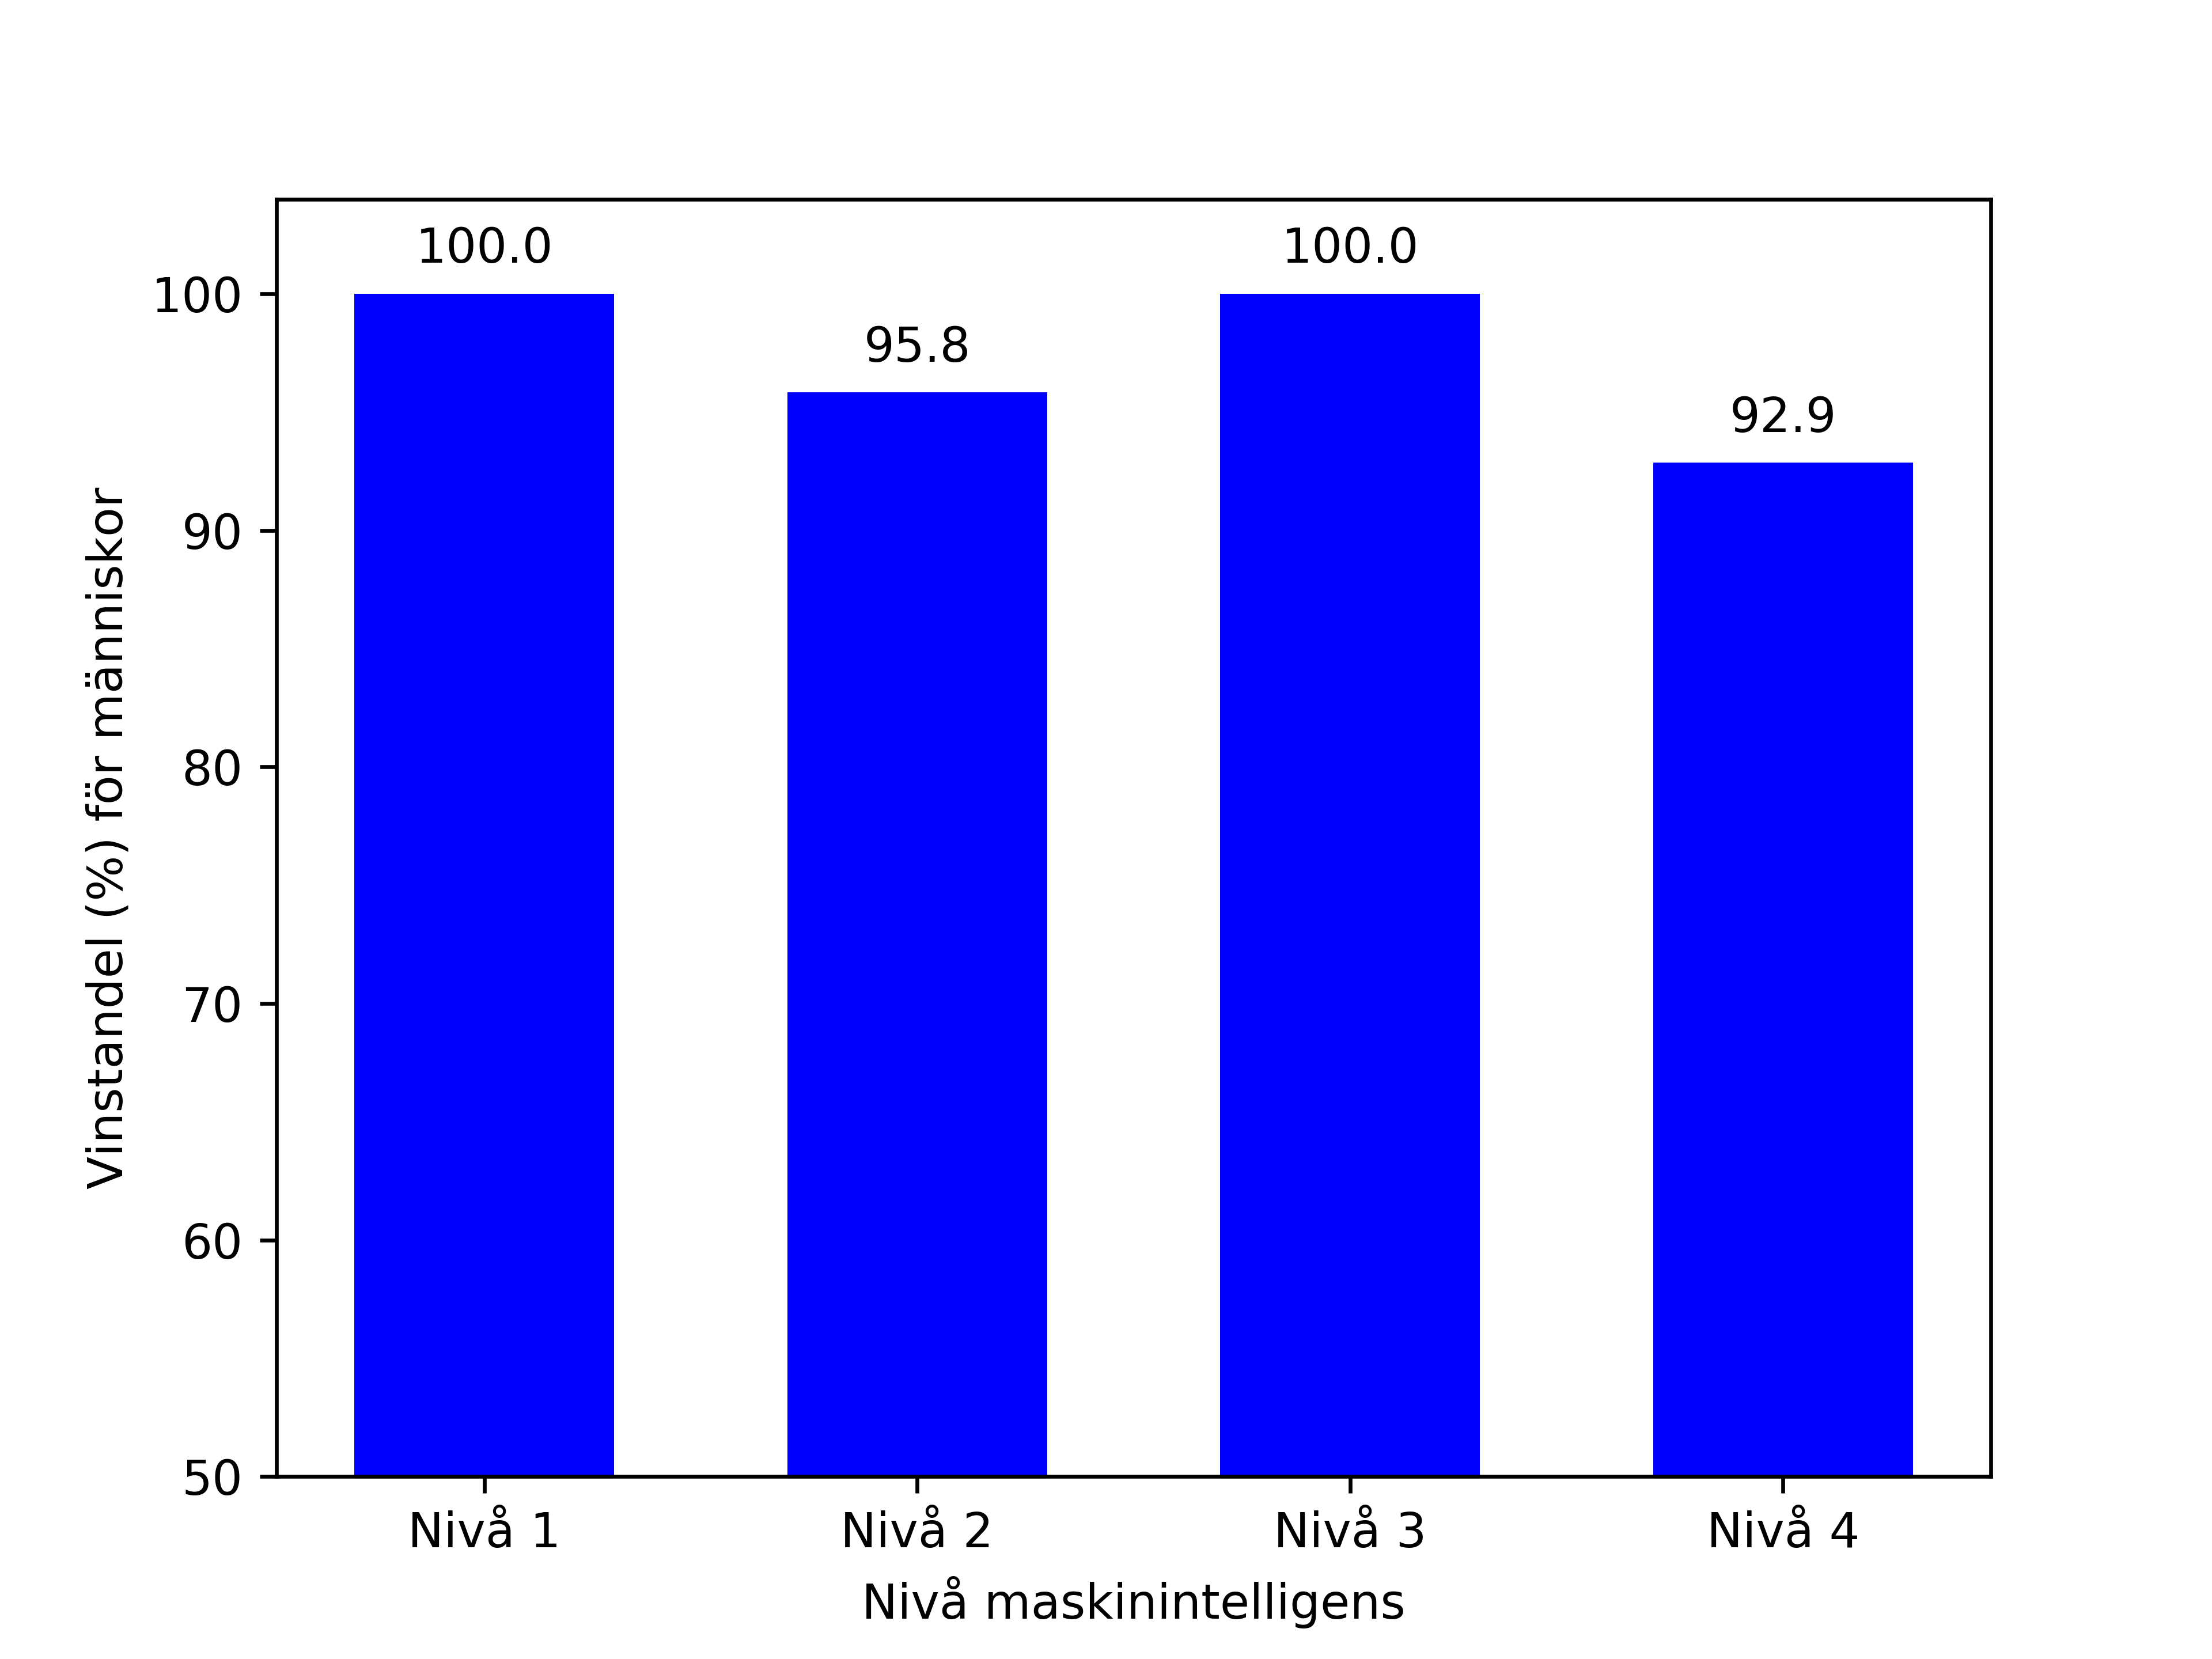
\includegraphics[height=3.5in]{./images/vinstandel_manniskor.png}
      \caption{Figuren visar på hur stor andel av spelade spel som människa vinner mot maskinintelligens av en given nivå.}\label{fig:vinstandelmanniskor}
    \end{figure}
    
    
    \begin{figure}[H]
      \centering
      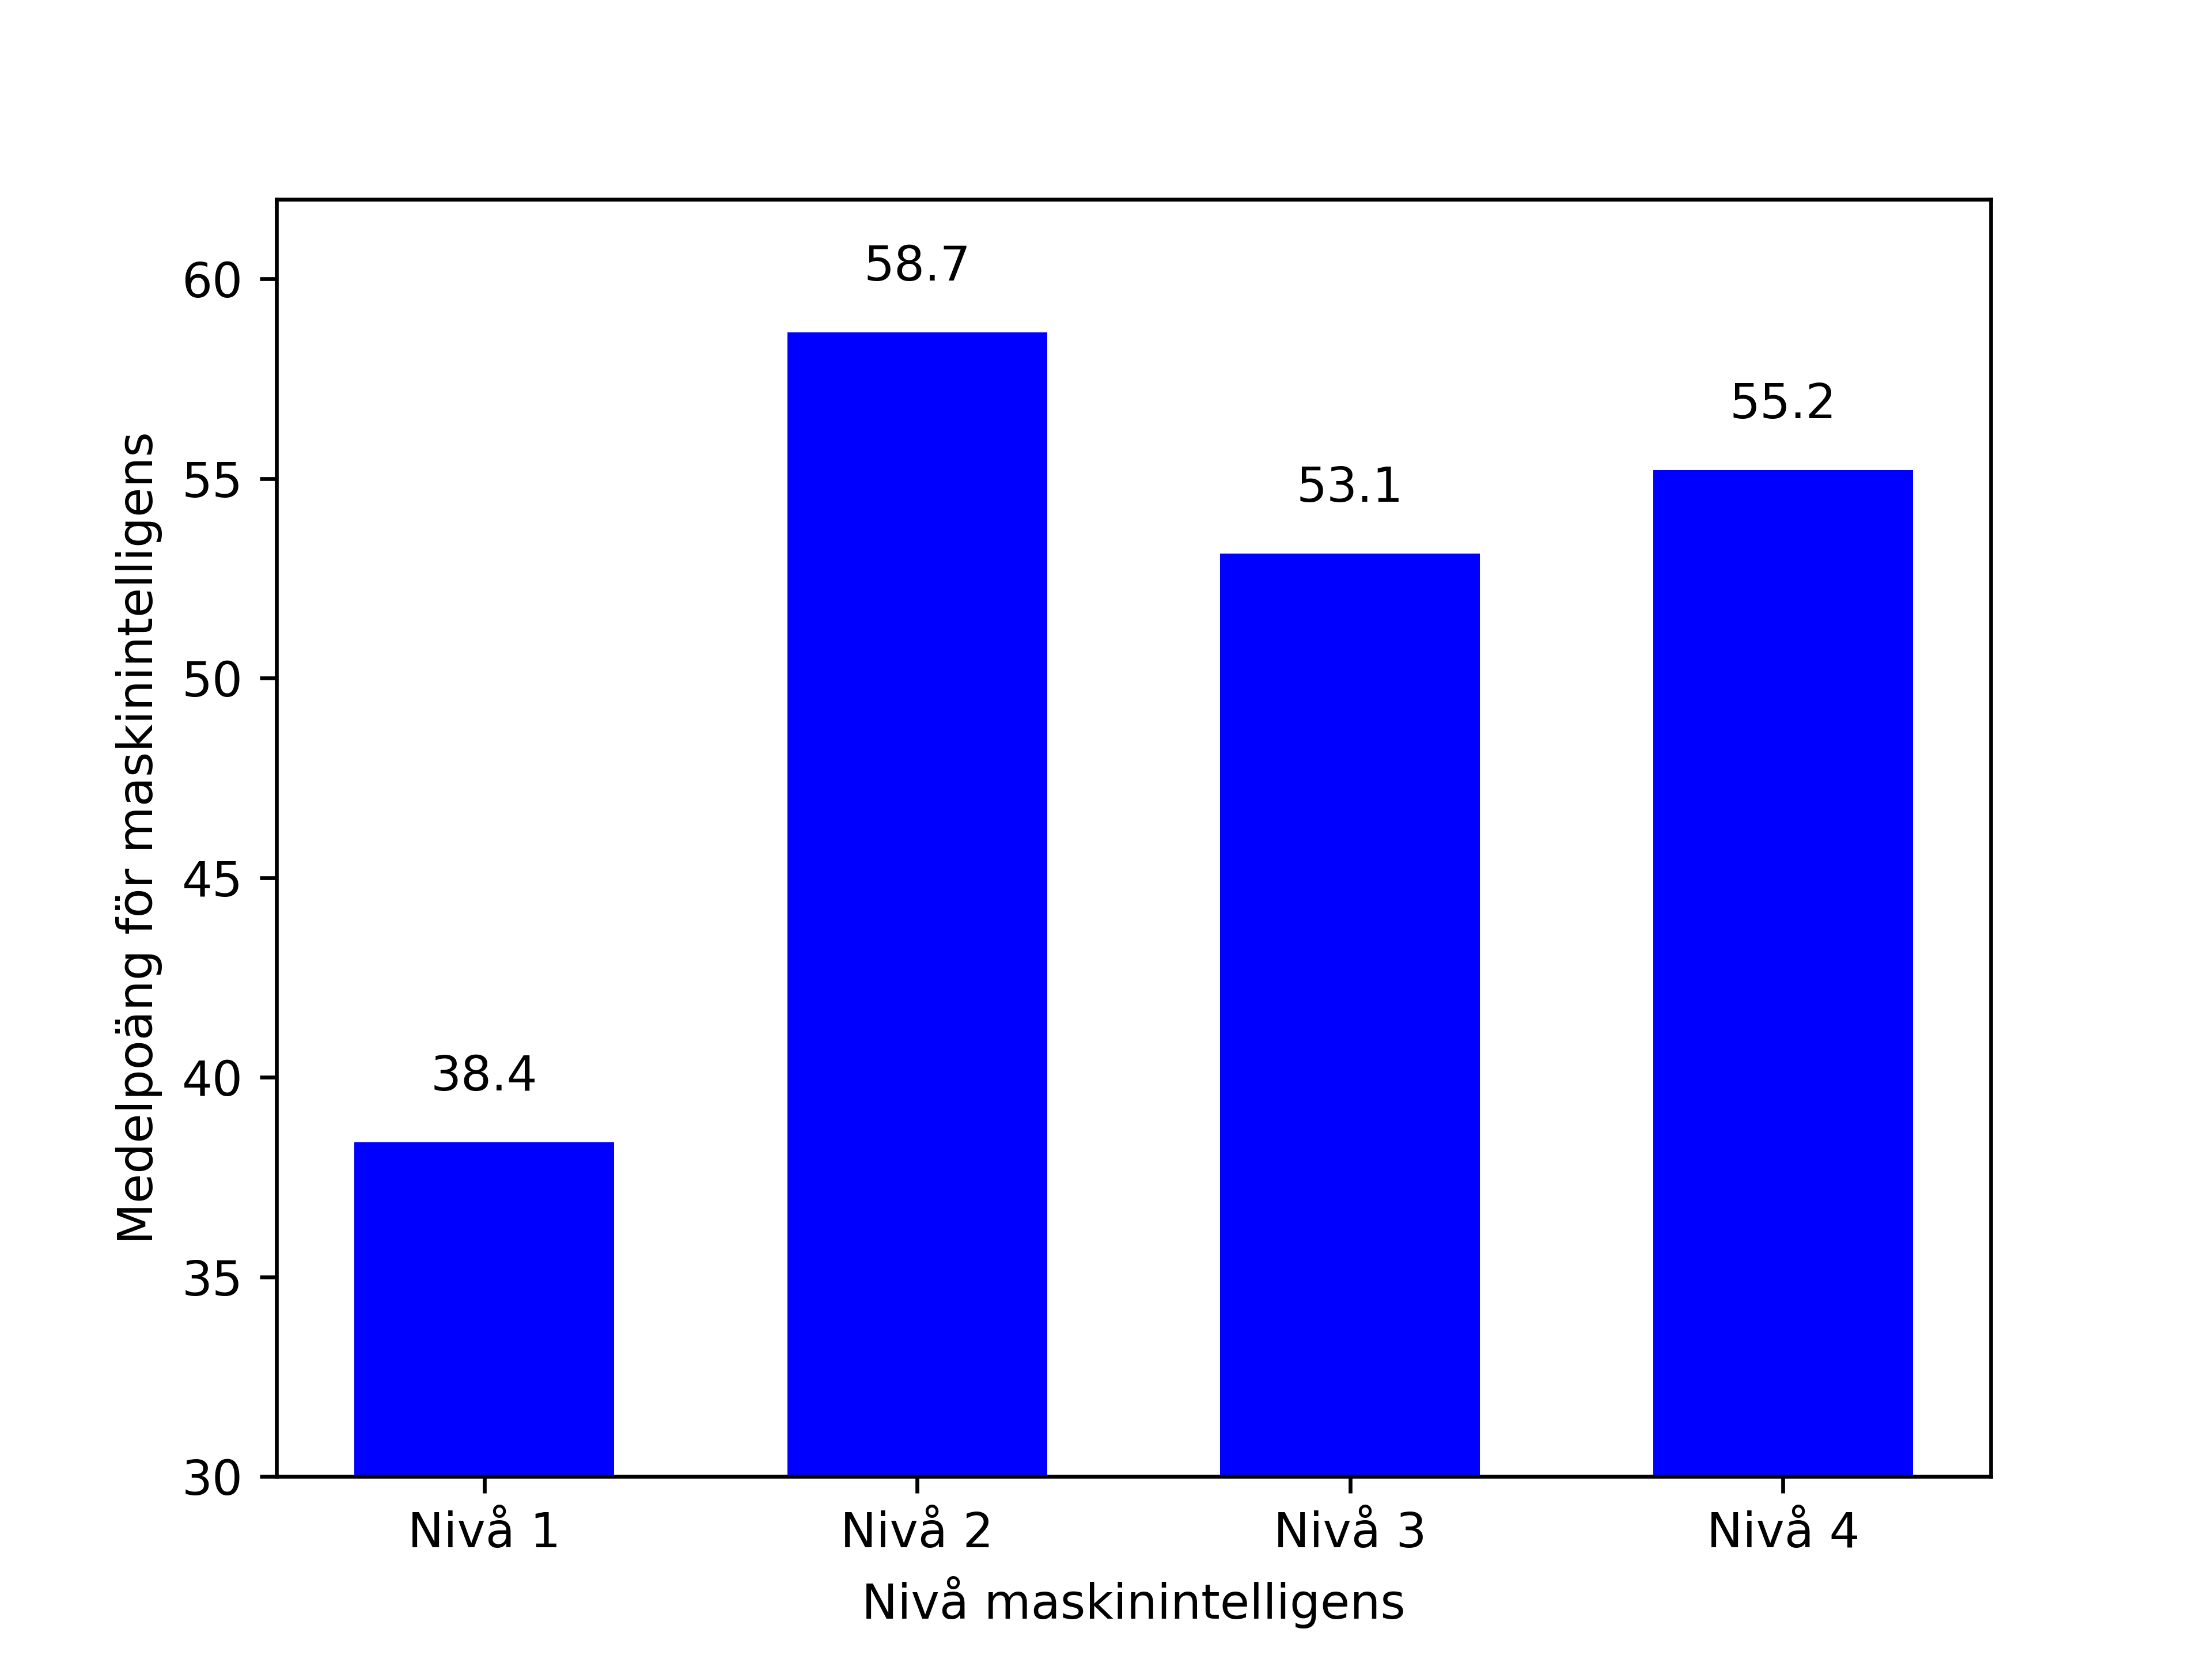
\includegraphics[height=3.5in]{./images/medelpoang_maskinintelligens.png}
      \caption{Figuren visar medelpoängen för en maskinintelligens av en viss
      nivå då den mötte människor.}\label{fig:medelpoangmaskinintelligens}
    \end{figure}

    
    \begin{figure}[H]
      \centering
      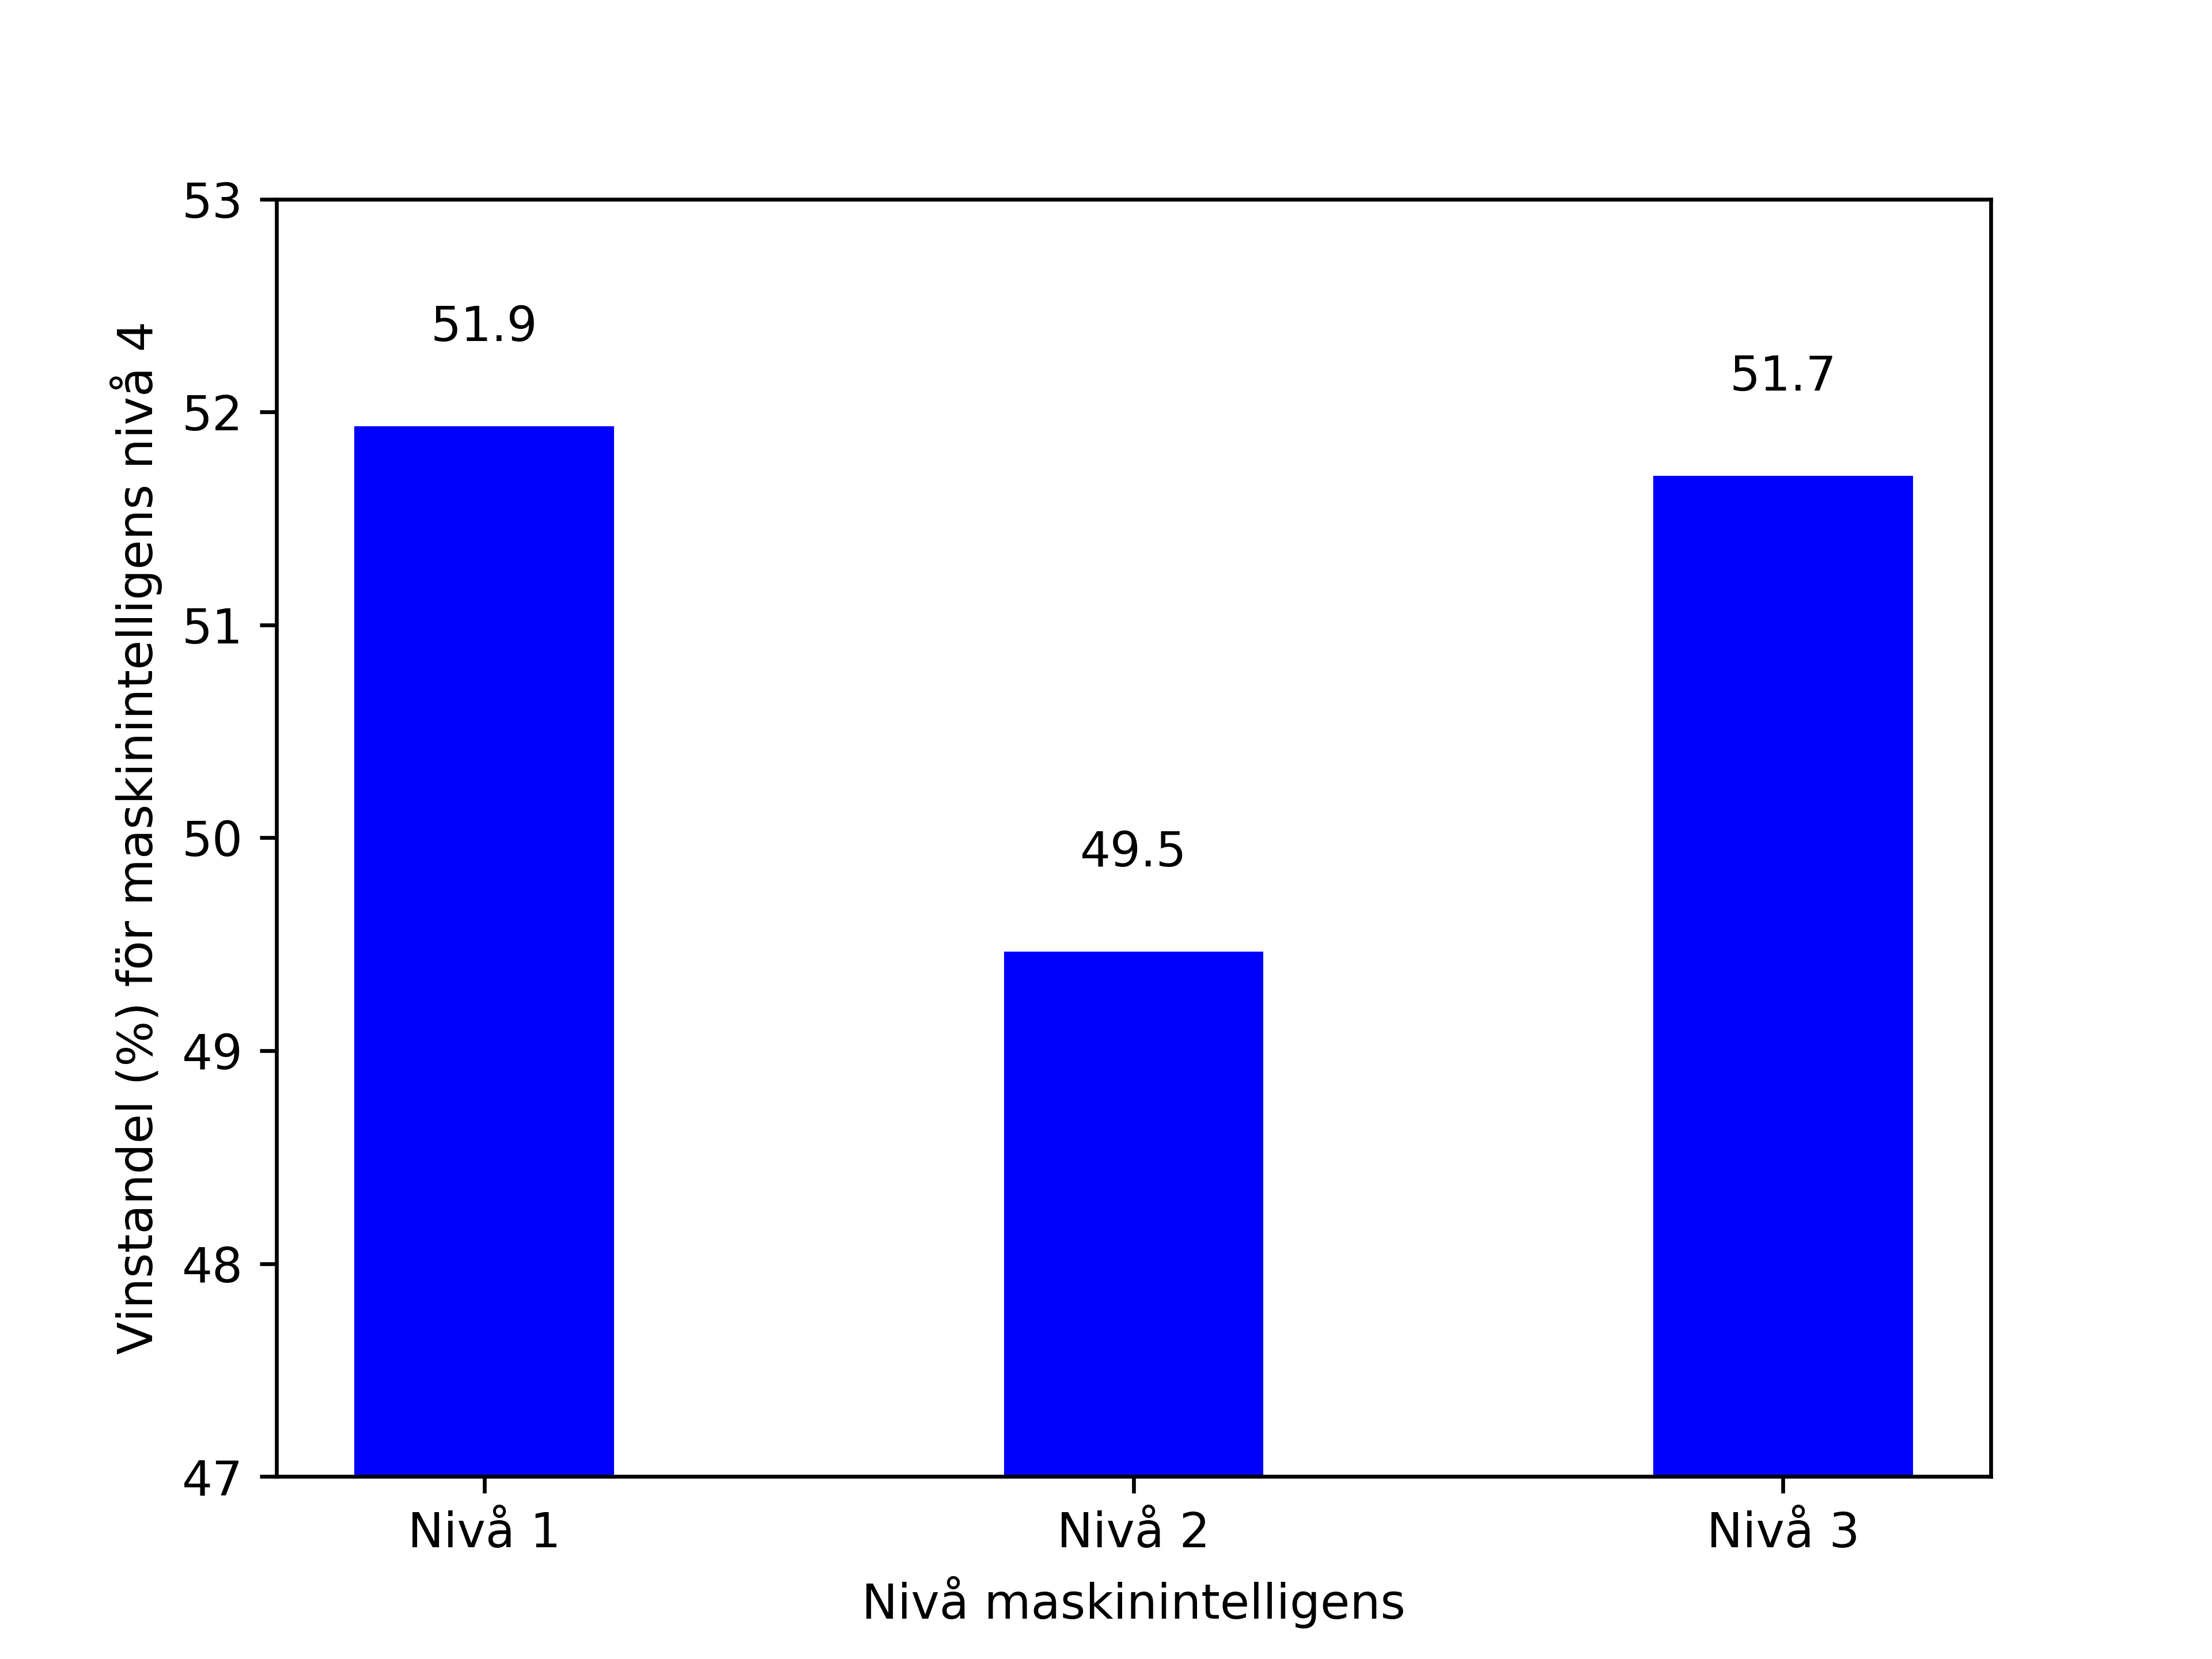
\includegraphics[height=3.5in]{./images/vinstandel_niva4.png} \caption{Figuren visar vinstandelen i procent för maskinintelligens nivå 4 då den möter en maskinintelligens av en given nivå.}\label{fig:vinstandelniva4}
    \end{figure}
  % --- End resultat --- %


  % --- Begin diskussion och slutsats --- %
  \section{Diskussion och slutsats}\label{sec:diskussionochslutsats}
  Figur 1 visar på att maskinintelligensen ej är bättre än människor på tärningsspelet \emph{Etthundra}. Även om maskinintelligens \emph{nivå 4} vinner flest spel kan ingen slutsats dras från denna figur förutom att människor är bättre än maskinintelligensen. Detta då resultatet baseras på en relativt liten mängd spel samt att skillnaden i vinstandel är liten. 
  
  Däremot visar figur \ref{fig:medelpoangmaskinintelligens} att maskinintelligensen blir bättre då den har tränat fler spel. Detta reflekteras i att medelpoängen maskinintelligensen ackumulerar under ett spels gång ökar i takt med att maskinintelligensen tränat fler spel. Överlägset sämst är maskinintelligens \emph{nivå 1} vars medelpoäng är 38,4. Marginellt bäst presterar maskinintelligens \emph{nivå 2}. Denna data är mer tillförlitlig än datan i figur \ref{fig:vinstandelmanniskor} då poängackumulation är mer nyanserat än en vinst eller en förlust. Man kan förlora ett spel med 1 poäng eller med 100 poäng. Bilden av maskinintelligensernas prestation blir således mer detaljerad eftersom man får poäng oftare än man vinner eller förlorar och därför kan figur \ref{fig:medelpoangmaskinintelligens} anses mer tillförlitlig än figur \ref{fig:vinstandelmanniskor}. 

  Figur \ref{fig:vinstandelniva4} förstärker datan i figur \ref{fig:medelpoangmaskinintelligens} då denna också pekar på att maskinintelligens \emph{nivå 2} är den som presterar bäst. Det enda som talar emot detta är figur \ref{fig:vinstandelmanniskor}, där \emph{nivå 4} presterar bäst, men som tidigare nämnts baseras den på minst mängd data och är därför minst tillförlitlig när man ska jämföra de olika nivåerna av maskinintelligens mot varandra. 

  Eftersom maskinintelligensen enbart tränade emot en annan maskinintelligens som hade tränat lika mycket som den själv, lär den sig hela tiden av att spela mot någon som är lika bra, marginellt sämre eller marginellt bättre än sig själv. Detta betyder att den får belöningar för drag och/eller kombinationer av drag som inte skulle lett till en vinst om den mötte en bättre spelare. Maskinintelligensen lär sig därför att spela dåligt, då det räcker med att spela dåligt för att vinna över en sämre motståndare. Det skulle därför vara bättre om maskinintelligensen fick träna mot en väldigt bra motståndare redan från början. Då skulle den lärt sig vad som fungerar och vad som inte fungerar när man möter en bra motståndare, inte vad som fungerar mot en dålig motståndare. Det bästa hade varit om maskinintelligensen fått träna genom att spela mot människor. Maskinintelligensen hade då lärt sig vad som är ett bra sätt att spela mot människor respektive vad som är ett dåligt sätt att spela mot människor. Detta är dock orimligt då maskinintelligensen behöver träna flera miljoner spel för att komma upp i en rimlig nivå. Om man räknar lågt och antar att ett \emph{Etthundra} spel tar en minut att spela och att maskinintelligensen konsekvent kan slå människor efter \emph{1 miljon} tränade spel, skulle det behövas 695 dagars kontinuerligt spelande för att uppnå detta. Det näst bästa alternativet hade varit att spela mot logik baserat på det optimala sättet att spela \emph{Etthundra}. Då hade maskinintelligensen fått möta en perfekt “spelare” och hade således behövt lära sig att spela på en väldigt hög nivå för att ha en chans att vinna.

  En annan förbättring hade varit att experimentera med $\varepsilon$-värdet. $\varepsilon$-värdet bestämmer hur snabbt stegringen går från att maskinintelligensen slumpmässigt bestämmer alla sina drag under träningen, till att alla dess drag är beräknade. Om detta värdet är för lågt, leder det till att maskinintelligensen slutar att slumpmässigt välja sina drag tidigt och därför hinner den ej utforska många och utvärdera många olika positioner. Dess beräknade drag baseras då på en liten mängd data. Maskinintelligensen saknar med ett lågt $\varepsilon$-värde erfarenheter och har därför inte tillräckligt med kunskap för att ta bra beslut. Om $\varepsilon$-värdet däremot är för högt kommer maskinintelligensen ta längre tid på sig innan den slutar att slumpmässigt välja sina drag. Detta är i sig självt inget dåligt, särskilt inte om maskinintelligensen hela tiden tränar mot en stark motståndare, då leder enbart ett högt $\varepsilon$-värde till att träningsprocessen tar längre tid. Om det istället är så att det är två maskinintelligenser som möter varandra, är ett för högt $\varepsilon$-värde dåligt. Detta då maskinintelligensen och dess motståndare båda kommer att välja sina drag slumpmässigt länge och de lär sig då att spela mot en motståndare som spelar slumpmässigt. Experimentation med $\alpha$ och $\gamma$-värden i SARSA-algoritmen (se \ref{subsubsec:sarsa}) hade även kunnat ge ett bättre resultat. 
  % --- End diskussion och slutsats --- %


  \cleardoublepage


  % --- Begin källförteckning --- %
  \bibliographystyle{plainnat}
  \bibliography{./references/gymnasiearbete_etthundra.bib}
  \addcontentsline{toc}{section}{\numberline{}Källhänvisning}
  % --- End källförteckning --- %


  \cleardoublepage


  % --- Begin bilagor --- %
  \appendix
    % --- Begin qtable --- %
    \section{Q-table - exempel}\label{tab:qtable}
      \begin{table}[H]
        \centering
        \caption{Exempel på hur ett Q-table kan se ut. Värdena är påhittade.}
        \begin{tabular}{l c r}
          \textbf{Poäng} & \textbf{Slå} & \textbf{Stanna} \\ \hline
          40 - 23 - 7    & 30,32        & 10,2            \\
          40 - 23 - 12   & 20,74        & 23,12           \\
          52 - 46 - 0    & 40,85        & 8,39            \\
          52 - 46 - 6    & 32,16        & 13,43           \\
        \end{tabular}
      \end{table}
      Kolumnen längst till vänster beskriver hur positionen ser ut. Exempelvis beskriver den andra raden (40-23-7) att spelaren har 40 poäng, att motståndaren har 23 poäng och att spelarens temporära poäng är 7. De två andra kolumnerna visar ett värde baserat på hur bra datorn tycker det är att göra respektive drag, slå eller stanna. När datorn utvärderas för att se hur bra den presterar slumpar den ej sina drag utan baserar enbart sina drag på värdena i kolumn två och tre. Exempelvis skulle datorn i positionen 40-23-12 välja att stanna då 23,12 är större än 20,74.
    % --- End qtable --- %
    % --- Begin data och kod --- %
    \section{Data och källkod}\label{app:data}
      Datan och källkoden för denna undersökning ligger uppe på GitHub: \\

      https://github.com/Zelmyx/Gymnasisearbete-Etthundra
    % --- End data och kod --- %
  % --- End bilagor --- %


\end{document}
